\section{Reproducible examples and verification status}
\label{sec:computations}

\subsection{An exact certificate with an infinite tail}

Consider the infinite multiset
\[
 1,\quad \tfrac12,\quad \tfrac12,\quad \tfrac14,\quad
 \tfrac1{16},\quad\tfrac1{32},\quad\tfrac1{64},\ldots.
\]
Its moments are the exact rational numbers
\begin{equation}\label{eq:modelmoments}
 p_j=1+2\left(\tfrac12\right)^j+\left(\tfrac14\right)^j
       +\frac{(1/16)^j}{1-2^{-j}}\qquad(j\ge1).
\end{equation}
The final fraction includes every tail occurrence. No truncation of an
infinite sum is used in the example.

Take centers $(1,1/2,1/4)$, radii $(1/20,1/40,1/80)$ and threshold $1/8$.
The exact rational checker first succeeds at $K=25$ when scanning upward
from one. Only $p_{25},\ldots,p_{31}$ enter this certificate. Its bound on
the missed count is approximately $0.7219569302<1$, so the missed count
is zero. The exact count intervals contain precisely the integers
$(1,2,1)$; their error radii are approximately
\[
 9.93\cdot10^{-29},\qquad 1.11\cdot10^{-19},\qquad
 4.33\cdot10^{-12}.
\]
These decimal displays summarize exact rational inequalities recorded in
\nolinkurl{artifacts/certificate_results.json}.

\begin{figure}[htbp]
 \centering
 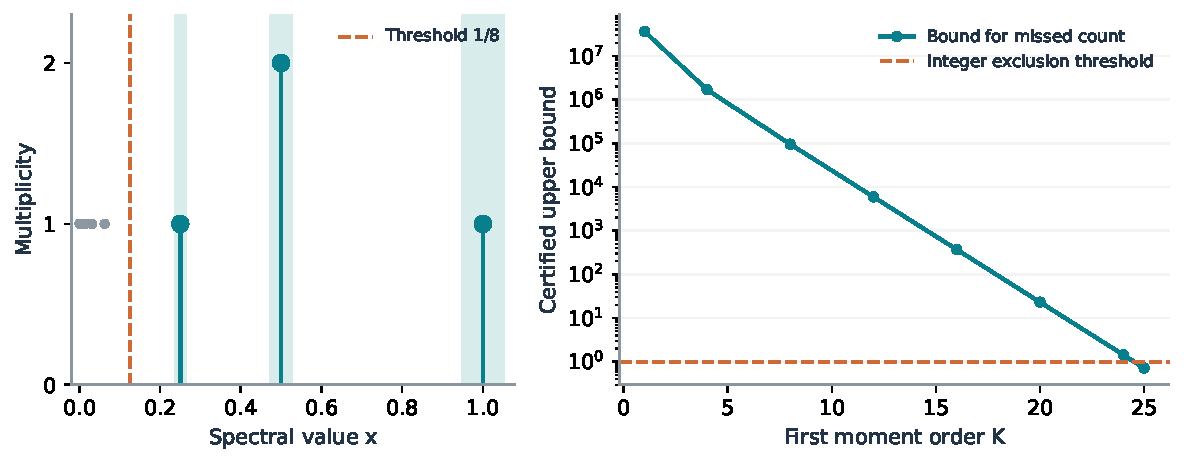
\includegraphics[width=\linewidth]{figures/certificate_example.pdf}
 \caption{Left: the exact model, with proposed intervals shaded and the
 threshold marked. Several tail points are displayed, but the calculation
 uses the whole tail. Right: the no-missing bound decreases below one at
 $K=25$. Local integer counts can already be determined at smaller $K$;
 certifying completeness is a separate requirement.}
 \label{fig:certificate}
\end{figure}

The same program verifies valid moment enclosures rounded to 36 decimal
places. It also verifies those enclosures after signed $10^{-20}$
perturbations of the candidate centers. Deliberately omitting the $1/2$
cluster fails the certificate, as do coarse moment enclosures rounded to
16 decimal places. A failed certificate is inconclusive about the
mathematical statement; it means that these particular sufficient bounds
do not prove it. In the omitted-cluster case, the proposed completeness
statement is in fact false.

The verifier accepts a JSON file containing centers, radii, a positive
integer $K$, a threshold, and a midpoint/error pair for every needed moment.
It forms the residual and count polynomials, evaluates their linear
moment functionals, and performs the interval and integer tests.
Every decision uses Python's \texttt{fractions.Fraction}. The program
rejects binary floating inputs and non-integer values of $K$.
It does not use a numerical root solver or invert a moment matrix.

\subsection{A zeta illustration, with its numerical status made explicit}

The separate program \texttt{code/zeta\_demo.py} applies the formulas to
the scaled nodes $y_n=200/(\tfrac14+\gamma_n^2)$.
It computes logarithmic Taylor coefficients of $H(200w)$ by discrete
Cauchy extraction on $|w|=1/16$, using 100-decimal-digit arithmetic and
96- and 128-point grids. Moments are obtained from the completed zeta
function, not from a truncated list of zeros. A call reporting the first
zero is used only for a diagnostic comparison.

With
\[
 K=16,\qquad a=0.99979776674462794831,\qquad
 r=0.05,\qquad \tau=0.7,
\]
the illustrative results are
\begin{center}
\begin{tabular}{@{}lr@{}}
\toprule
Quantity & Numerical value\\
\midrule
$p_{16}$ & $0.996772251654086920874827$\\
$p_{17}$ & $0.996568982997367045027571$\\
$p_{18}$ & $0.996366681112969093653953$\\
Residual $R_{16}$ & $9.25323237789\cdot10^{-7}$\\
Count estimate $S$ & $1.00003019414010$\\
Formula for count-error radius $CR_{16}$ & $0.000668452280241$\\
Formula for missed-count bound & $0.111374257031$\\
\bottomrule
\end{tabular}
\end{center}
The inverse-coordinate interval corresponds to the ordinate interval
$(13.7935812554,14.5024529500)$, and the threshold corresponds to height
$16.8956883765$. Were the input moment values accompanied by sufficiently
tight certified enclosures, these margins would certify exactly one zero
in that interval and no other positive-ordinate zero below the height.

This run is \textbf{a numerical illustration, not a certified zeta-zero
count}. The \texttt{mpmath} special-function evaluations have not been
enclosed by rigorous ball arithmetic. Agreement between grids cannot
replace such enclosures. The general theorem is proved independently of
this run; the preceding infinite-tail model is checked exactly.

For clarity, the quadrature discretization itself has a simple analytic
bound. If $M>j$ samples are used on radius $R$ and $q=p_1R<1$, then the
exact-arithmetic extracted moment obeys
\[
 |\widetilde p_j-p_j|\le p_1^j\frac{q^M}{1-q^M}.
\]
Indeed $[w^n]\log H(w)=(-1)^{n-1}p_n/n$, $p_n\le p_1^n$, and the
discrete sum aliases only indices $j+\ell M$. In this numerical run
$q\approx0.2887$ and $|H(200w)-1|\le e^q-1<1$, which justifies the
principal logarithm on the contour. The reported evaluations of the
analytic alias bound are still numerical values, not outward-rounded
certified upper endpoints.

\subsection{Exact determinant and surgery checks}

\texttt{code/determinant\_verify.py} uses exact integer determinants and gcds.
It checks Cauchy--Binet, all maximal minors, and the asserted bounds for the
four rank-two equality matrices and the rank-three complementary example.
Their Gram determinants are $24,12,8,7,24$. An optional finite enumeration
of 19,600 unit-minor normal-form triples provides an additional diagnostic;
the proof of Theorem~\ref{thm:determinant} does not rely on that enumeration.

\texttt{code/surgery\_verify.py} checks the exact rational Newton identities,
the positive disjoint root brackets, and the vanishing of the first three
coefficients of the numerator-minus-denominator polynomial in $t^2$ for
the sine-product example of Section~\ref{sec:surgery}. Thus the finite
algebra giving Taylor agreement through order five is independently
reproducible. The infinite-product statements are proved in the text.

\subsection{A practical formalization route}

No new theorem in this note is represented as already checked by Lean.
The exact programs are ordinary executable arithmetic; they are neither
kernel proofs of the analytic arguments nor a rebuild of the upstream
development. A reasonable Lean implementation would proceed in the
following order.

\begin{enumerate}
\item Formalize the four- and five-label integer Pl\"ucker lemmas. Their
proofs require elementary inequalities, finite case splits, and a modulo-three
double count. Lift them through finite incidence sums, Cauchy--Binet and
complementary minors to Theorem~\ref{thm:determinant}.
\item Prove the rational polynomial identities for $P,L_i,Q_i$ and a
finite-support version of Theorem~\ref{thm:residual}. The noise propagation
and integer-rounding corollary are algebraic and order-theoretic.
\item Prove the pointwise Taylor-remainder estimate for $h_i$ on a positive
interval, then pass from finite sums to a summable positive spectrum using
the boundedness $x_n\le p_1$.
\item Connect the completed zeta product and the symmetry quotient to the
standard Mathlib zeta function, using the upstream RH theorem only at the
zero-reality step. A rigorous numerical front end must supply certified
moment enclosures before the rational checker can certify actual zeta data.
\item Formalize the surgery construction either through the local inverse
theorem or through Newton identities and polynomial endpoint signs.
The latter has a small finite certificate interface.
\end{enumerate}

\section{What is proved, and what remains a research claim}

The results in this note have complete mathematical proofs. The spectral
certificate is unconditional for a positive summable integer spectrum;
its zeta specialization uses RH. The determinant bound and finite-factor
surgery theorem are independent of RH. Exact rational examples check the
finite arithmetic, and separate mathematical reviews checked the key
constant calculations, incidence counts, normalization, and boundary cases.
The note has not undergone external peer review.

The proposed novelty is specific: the explicit infinite-tail cluster
certificate and its error/termination theorem; the aggregate
squared-minor bound with a penalty for vanishing minors; and the particular
balanced real-zero surgery preserving an exact finite jet and the eventual
zero-counting function. The ingredients are classical. Targeted primary
literature searches identified close results and are discussed in the
relevant sections. They cannot establish that no equivalent formulation
has appeared elsewhere.

These statements do not resolve global simplicity, pair correlation,
the Lindel\"of hypothesis for unrelated $L$-function families, or a broader
version of GRH. They are concrete proved results and reusable certificates
derived from the two supplied sources, with their dependencies and
computational limits specified.
